\chapter{General discussion}
\label{chap:general-discussion}

In this chapter I begin by describing the landscape-scale phenotyping prototype and its components. The prototype components are the result of research on phenology modelling (Chapter \ref{chap:phemology}), uncertainty estimation (Chapter \ref{chap:uncertainty}), \gls{RTM}-based crop trait retrieval (Chapter \ref{chap:insights}) and crop growth reconstruction (Chapter \ref{chap:drc}). After describing the prototype, I focus on the three research questions formulated in the Introduction (Chapter \ref{sec:intro-obj-rj}) and the role of prior knowledge from field phenotyping. I also show how the prototype could contribute to research and applications in precision agriculture, phenotyping research, and global food security. Beyond these considerations, I discuss open questions and directions for further research needed to advance the science of landscape-scale phenotyping systems.

\section{A prototype for landscape-scale phenotyping}
Figure \ref{fig:oa-disc-prototype} shows a sketch of how the individual research components can be transferred to a landscape level prototype to quantify winter wheat growth and development.

The main data sources for the prototype are environmental covariates, mainly air temperature, and high resolution optical satellite imagery from the \gls{S2} mission. The necessary calibration of the prototype is mainly based on field phenotyping data, which encode the relationships between development and growth (see Chapter \ref{chap:insights}) and between plant growth and environmental conditions (Chapter \ref{chap:drc}). These calibration data thus represent the physiological and phenological knowledge of G $\times$ E interactions in crops in general and wheat in particular. Using the calibration and the two data sources, the functionality of the prototype can now be demonstrated in three components.

\subsection{Components}

\paragraph{Component 1 -- Timing and duration of key phenological stages}
The first step is to determine the timing of key phenological development stages as described in Chapters \ref{chap:phemology} and \ref{chap:insights}. This is important to determine the onset and duration of the \gls{SE} period, which was the main focus of this thesis due to its importance for crop productivity and grain yield formation \citep{gonzalez_grain_2003, fischer_wheat_2011}, as explained in Chapter \ref{chap:introduction}. The phenology model uses day length and weather data and has a coarse spatial resolution (km scale) due to the resolution of most meteorological data products at the landscape scale. The timing extracted from the phenology model will therefore limit the period over which satellite data should be considered.

\paragraph{Component 2 -- Trait retrieval from satellite imagery}
Once the relevant time period has been extracted from the phenology model, satellite data are searched and converted to \gls{GLAI} using physiological and phenological priors from field phenotyping as described in Chapter \ref{chap:insights} using RTM inversion and the software \gls{EOdal} (Chapter \ref{chap:eodal}). Thus, for each cloud-free \gls{S2} scene, \gls{GLAI} estimates are available at 10 $\times$ 10 m spatial resolution. This allows spatial detail to be resolved, e.g. on within-field heterogeneity, which, as noted above, is not available from the temperature data. The \gls{GLAI} estimates based on the \gls{S2} data are thus snapshots of the apparent growth conditions.

\paragraph{Component 3 -- Reconstruction of growth}
In the third component, growth dynamics during the \gls{SE} period are modelled at high spatial (10 m) and temporal resolution (hourly or daily). For this purpose, \gls{S2} \gls{GLAI} observations and air temperature records are combined using the \gls{DRC}s described in Chapter \ref{chap:drc}. The \gls{DRC}s encode the physiological knowledge of the relationship between air temperature and leaf area dynamics. In addition, the uncertainty in the \gls{S2} \gls{GLAI} observation from the Chapter \ref{chap:uncertainty} is utilized. This is achieved by using a probabilistic data assimilation scheme that integrates temperature and satellite data.

\begin{figure}[H]
    \centering
    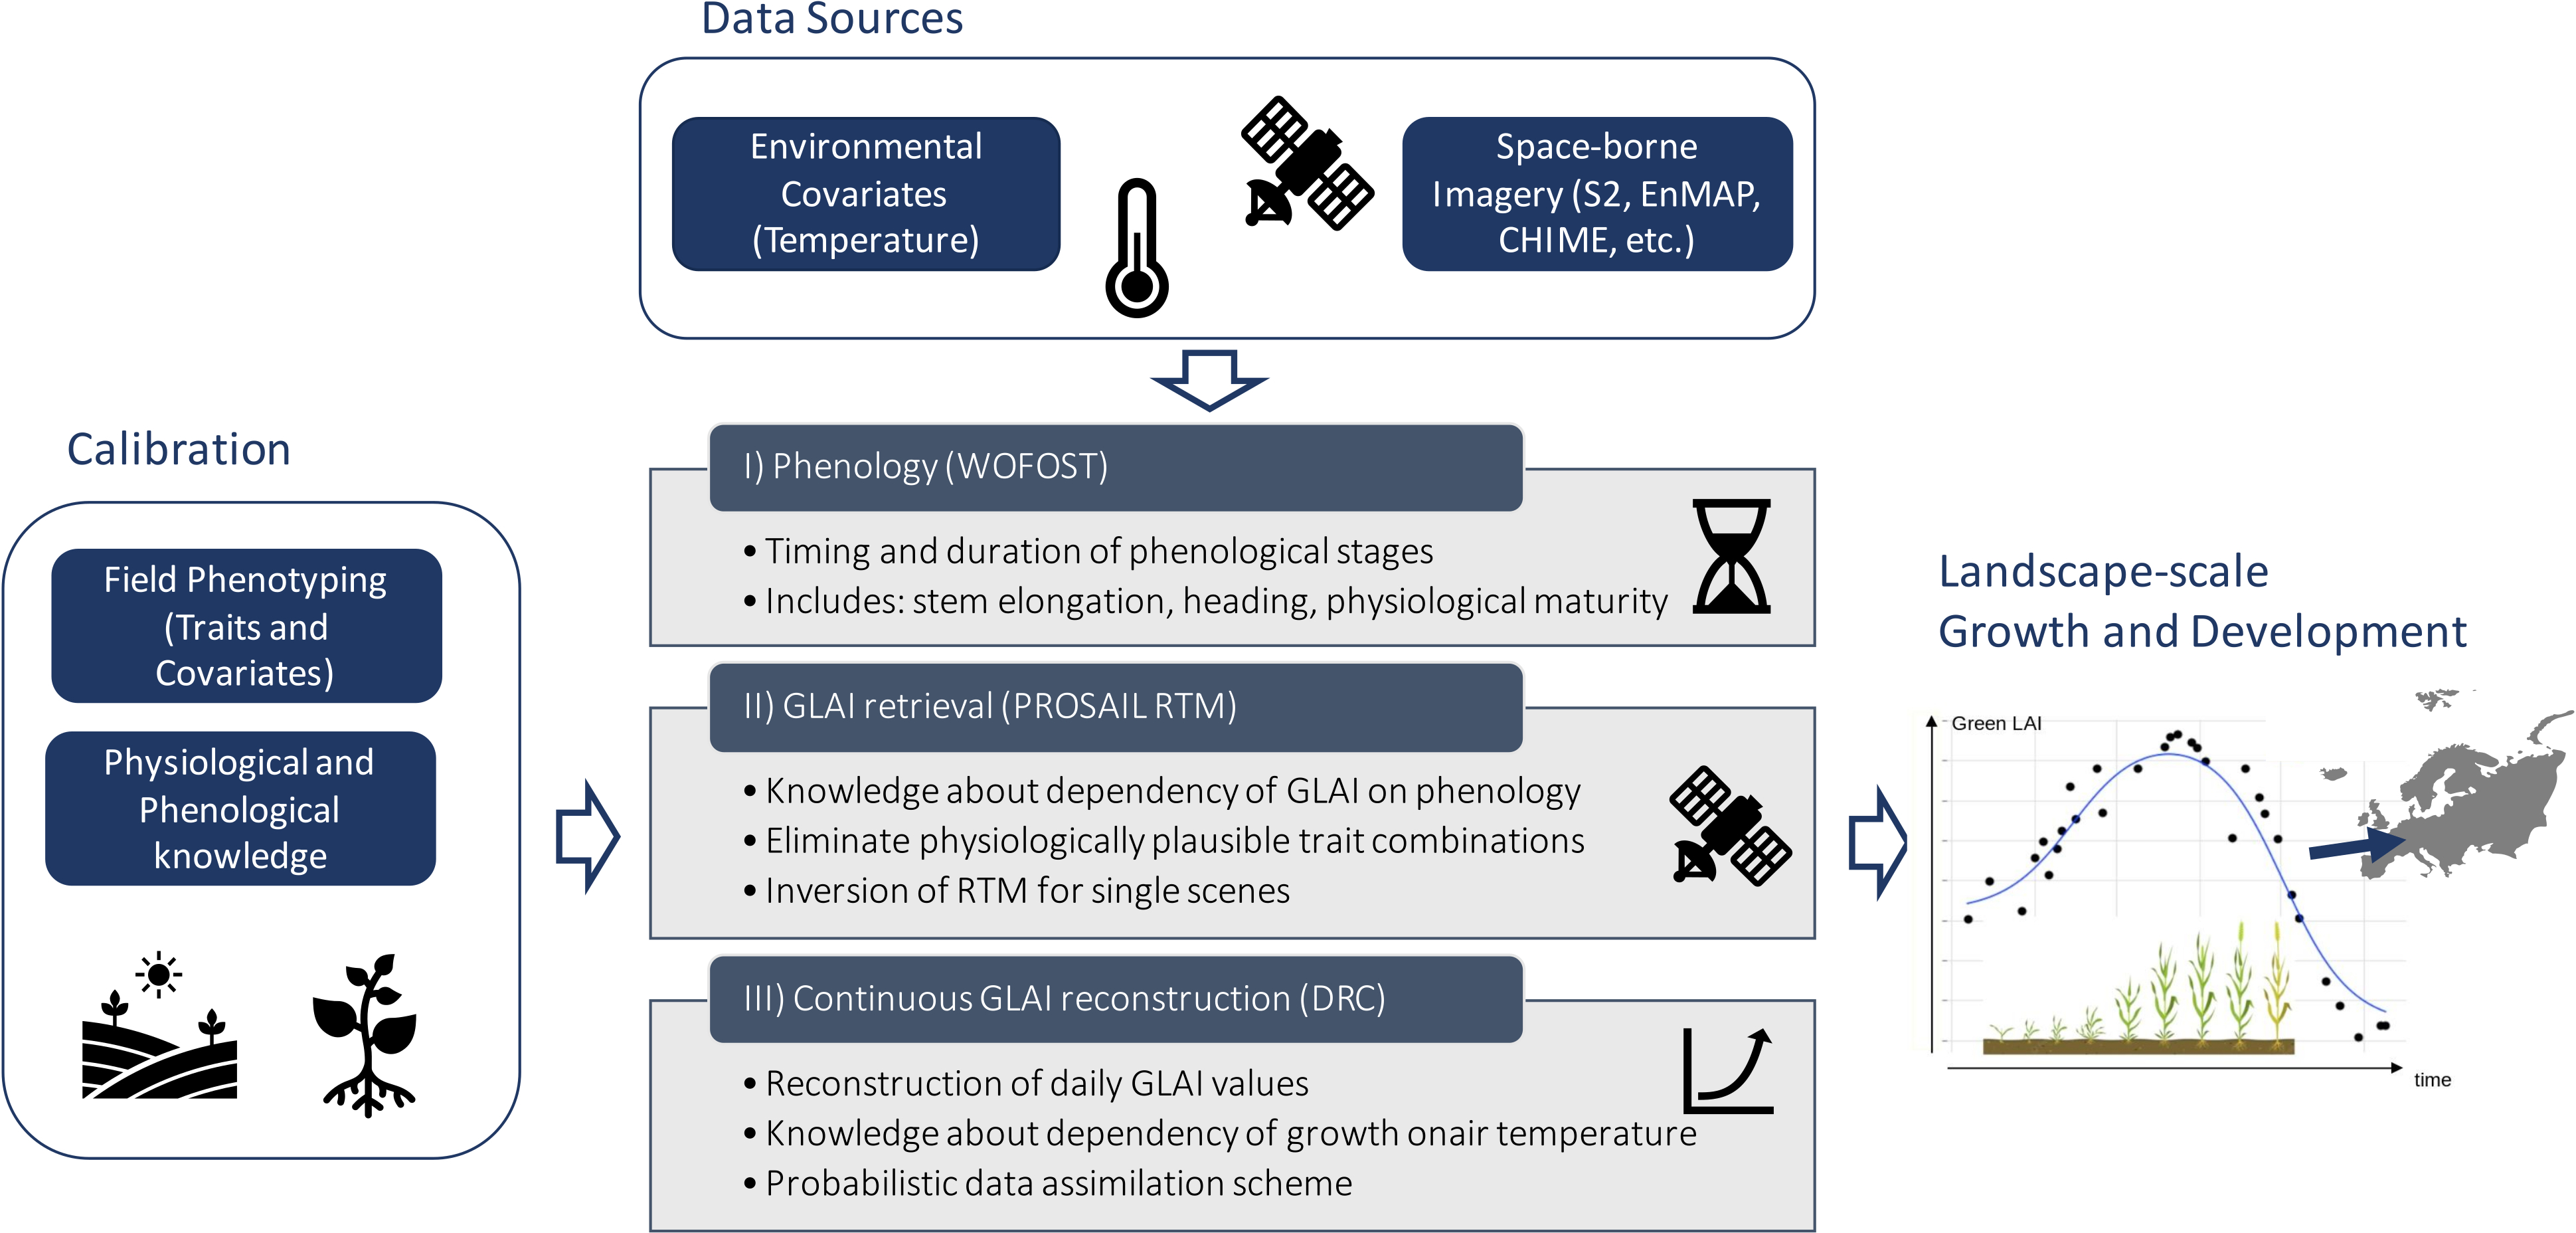
\includegraphics[width=\textwidth]{07-Discussion/img/prototype.jpg}
    \caption{The proposed prototype for landscape scale phenotyping of winter wheat growth and development as a key outcome of this thesis.}
    \label{fig:oa-disc-prototype}
\end{figure}

\section{Answers to research questions}

\subsection{Can field phenotyping provide prior knowledge to improve the relationship between radiative characteristics and crop traits?}
\label{subsec:oa-disc-aw-rq1}

Three methods were identified in this thesis that use prior knowledge from field phenotyping to improve the relationship between radiative characteristics and crop traits.

\begin{enumerate}

\item In Chapter \ref{chap:phemology}, a phenological model was calibrated using heading date ratings of two Swiss winter wheat varieties. The calibration data came from variety trials distributed across the Swiss Plateau, covering the years 2000 to 2018. The phenological model was then used to select satellite observations acquired during the \gls{SE} period (see Figure \ref{fig:oa-disc-prototype}). This does not improve the relationship between spectral properties and plant traits as such, but it is a necessary condition to narrow down the selection of relevant satellite scenes and to facilitate their interpretation. For example, the timing of the heading coincides with the timing of the maximum \gls{GLAI} (c.f., Figure \ref{fig:ww-growth-development}). If a \gls{GLAI} observation is available close to the modelled heading date, this \gls{GLAI} value is likely to be the maximum the crop reached during its development. Despite encouraging results, the phenological model operates at a coarse spatial resolution of 1 $\times$ 1 km and does not include environmental covariates other than air temperature and day length. This could be problematic in the case of small-scale differences in phenological development, e.g. due to microclimatic effects, or in situations where development is not limited by temperature alone, e.g. during droughts.

\item The second method is the use of physiological and phenological priors to constrain the \gls{RTM} inversion, as explained in Chapter \ref{chap:insights}. The phenological priors were mainly obtained from the FIP phenotyping site at Lindau-Eschikon (Switzerland, \cite{kirchgessner_eth_2017}) for the years 2015 to 2022. The physiological priors were mostly obtained from a single growing season in close proximity to the FIP site as part of Samuel Wildhaber's master's thesis \citep{wildhaber_assessing_2023}. Data from other sites in northern Switzerland and southern Germany were also included. However, the number of data points was small compared to the FIP data. Although the prior information improved the \gls{GLAI} retrieval from \gls{S2} images as shown in Chapter \ref{chap:insights}, the unbalanced calibration dataset may limit the geographical representativeness in terms of soil, climate, topography, and management. Similarly, observed shifts in phenology due to climate change (Chapter \ref{chap:phemology}) may not be well captured by a calibration dataset that contains only a small number of growing seasons. A larger calibration dataset with more sites and years would therefore be beneficial.

\item Similarly, the relationship between satellite derived \gls{GLAI} and growth as a dynamic trait was established in Chapter \ref{chap:drc} as a third method. Again, the calibration data relied mainly on the dataset from Samuel Wildhaber's master's thesis and field campaigns from southern and western Germany, limiting the total number of sites and years available. Although the \gls{DRC}s outperformed the baseline without physiological prior knowledge, the \gls{DRC}s failed to provide stable results for periods of prolonged cloud cover, which has been identified as a major drawback for a satellite-based phenotyping system \citep{zhang_high-resolution_2020}. In addition, the limited calibration dataset may not reflect extreme events such as high temperatures around $T_{max}$ well. As discussed in Section \ref{sec:drc_discussion}, this may explain the poor performance of the more sophisticated Wang-Engels \gls{DRC}.

\end{enumerate}

Overall, it is fair to say that field phenotyping datasets can provide prior knowledge to improve the relationship between radiative characteristics and crop traits. In principle, the prototype is transferable in space and time through the use of models based on physics (\gls{RTM}) and physiology.
However, it is crucial to have field phenotyping datasets with as many different site-year combinations as possible. A large number of sites increases the number of site conditions in terms of soils, climate and management. A large number of years per site is beneficial for studying the effects of weather patterns and increases the chance of including extreme weather events, which may become more relevant in a changing climate.

Therefore, a multi-experiment dataset spanning multiple sites and years, as suggested by \cite{smith_scaling_2021}, would be required for a more robust parameterisation of the prototype. Concepts such as the Global Agro-Environmental Stratification Zones \citep{muecher_new_2016} could help to design multi-experiment datasets and assess the representativeness of existing field phenotyping datasets, such as those from the FIP site.

\subsection{Can a landscape-scale phenotyping approach provide accurate, physiologically based and traceable insights into winter wheat growth and development?}

The quantification of uncertainties (see Chapter \ref{chap:uncertainty}) satisfies the requirement for traceability (Section \ref{sec:intro-obj-rj}). The integration of prior knowledge from field phenotyping satisfies the requirement for physiological plausibility, although the limitations outlined in Section \ref{subsec:oa-disc-aw-rq1} should be taken into account.

The accuracy of the methodology has been demonstrated using multi-year, independent in-situ data for phenological development (RMSE for heading date: 2 days, Chapter \ref{chap:phemology}) and GLAI (smallest relative error: 13\%, Chapter \ref{chap:drc}). As with the calibration data (see Chapter \ref{subsec:oa-disc-aw-rq1}), a larger validation dataset with more sites and years would be beneficial. Currently, the validation datasets contain only a limited number of sites and years, which may not fully represent the geographic variability of soil types and topography within the Swiss Plateau, as well as extreme weather events. Therefore, the full phenotypic plasticity of winter wheat genotypes may not have been fully captured.

The relative standard uncertainty in remotely sensed \gls{GLAI} values was found to take up to 5\% depending on the development stage of the crops (Chapter \ref{chap:uncertainty}). This uncertainty translated into an uncertainty in the timing of \gls{LSP} events in the magnitude of a few days. However, the uncertainty budget is still incomplete, i.e. it is likely to be higher than the figures reported here (see the discussion in Section \ref{sec:unc_discussion}). In addition, the uncertainty in field phenotyping data has not been addressed in this work. Therefore, further quantification of uncertainty in both satellite imagery and field phenotyping data is clearly needed. In addition, depending on the application, it should be clarified what range of uncertainty is considered acceptable. For breeding experiments, this is likely to be much narrower than for large-scale biomass estimates.

\subsection{What are the potentials but also the limitations and challenges of such a landscape phenotyping approach?}

The prototype allows the study of G $\times$ E interactions that could not be fully addressed by small-scale field phenotyping experiments. Such studies could include effects of changes in soil properties or topography that are spatially continuous and affect plant growth and development through soil water availability, exposure to wind and sunlight, or nutrient availability. In addition, the \gls{GLAI} estimates can be converted to biomass \citep{aase_relationship_1978} and -- in perspective -- grain yield, which are arguably important agronomic traits for decision making and policy advice. Accurate modelling of these traits will therefore not only advance the science behind \gls{EO}-based applications for agriculture, but also help to meet the needs of a growing world population.

The main obstacle to this potential is the lack of in situ data: Management data, in particular the sowing date or the variety used, is essential agronomic information that is not yet available on a large scale. In many countries, including Switzerland, the management data that the state is obliged to collect and publish include the main crop, but no further management data. In addition, research data from field phenotyping and variety testing, which are key to calibrating models, are often not publicly available. When they are, the data are often not standardised and poorly documented, so it is not clear how the data were collected and what the uncertainties are.

From a modelling perspective, there is room for improvement in the representation of canopy structure and morphology, which would further increase physiological plausibility. This is related to the discussion on the representation of vertical gradients in leaf number and \gls{Cab} in Chapter \ref{chap:insights}. Canopy vertical gradients also address other research questions, such as differences in the interception of incoming solar radiation between sunlit and shaded leaves under direct and diffuse light conditions \citep{he_development_2013}. Approaches using multiple vertically stacked canopy layers would greatly facilitate the representation of gradients and could be a viable method for modelling, for example, the succession of senescence within a canopy.

Another limitation of the prototype is its spatial resolution of currently 10 m. The pixel size of 10 m can cause spectral mixing problems close to field boundaries and make it difficult to resolve small-scale details such as flower strips, hedges or individual trees within a parcel. For small plots, it may not be possible to find a pure pixel, i.e. a pixel that is not affected by spectral mixing. \cite{meier_assessments_2020} found that, at a spatial resolution of 10 m, up to 6.4\% of all parcels (0.49\% of the total agricultural land area) were lost due to the lack of pure pixels, and for up to 50\% of the fields (10.53\% of the total agricultural land area) no site-specific agricultural applications were possible due to the small number of pure pixels ($\le$ 50 pixels). These figures were reported for Bavaria, which has a comparable average field size (1.6 ha) to Switzerland (1.4 ha) and a similar agricultural land use pattern. A solution to this problem could be the use of higher resolution data, such as from the Planet Labs$^{\circledR}$ constellation, with a pixel size of less than 5 m. In Samuel Wildhaber's master's thesis, it was shown that such high resolution data have potential for agricultural applications and could outperform \gls{S2} data when it comes to representing small-scale detail \citep{wildhaber_assessing_2023}. At the same time, unlike \gls{S2}, the data is proprietary and therefore more expensive to acquire. Deep learning based super-resolution may therefore be a more viable option to improve the spatial detail available from \gls{S2}, but research carried out by Julian Neff as part of his Master's thesis suggests that more effort may be required to achieve satisfactory results.

\section{Potential contributions}

\subsection{Precision farming}
An important precision farming measure is the site-specific application of \gls{N} fertiliser \citep{argento_site-specific_2021}. As Gregor Perich showed in his PhD thesis, \gls{S2} satellite derived estimates of \gls{GLAI} and \gls{CCC} can be used for site-specific estimation of \gls{N} nutritional status in crops \citep{perich_satellite-based_2023}. The retrieval of \gls{GLAI} and \gls{CCC} based on physiological and phenological priors from \gls{S2} imagery outlined in Chapter \ref{chap:insights} could therefore be used to improve the accuracy and reliability of satellite-based N fertilisation recommendations. In addition, the reliability of the \gls{N} application maps can be assessed using the uncertainties available in Chapter \ref{chap:uncertainty}.

Besides fertilisation, accurate and timely estimates of crop biomass and grain yield can help to optimise the allocation of resources and the application of management measures. The reconstruction of crop growth to anthesis presented in Chapter \ref{chap:drc} is a first step in this direction. From work co-authored by \cite{amin_-season_2024} we know that grain yield predictions for winter wheat can be made with confidence around the heading date. The timing of the heading date can be estimated thanks to the phenological model described in Chapter \ref{chap:phemology}. The \gls{GLAI} estimates at heading could therefore be converted into biomass using an empirical formula developed as part of Vilma Rantanen's bachelor's thesis. These biomass estimates could then be used as input for a predictive model to estimate grain yield up to two months before harvest.

\subsection{Phenotyping research}
Landscape-scale phenotyping systems composed of multi-experiment designs have been identified as a major need in phenotyping research to cope with the spatio-temporal variability of crop responses to abiotic stressors \citep{smith_scaling_2021}. Here, satellite remote sensing platforms have been proposed as a cost-effective, highly automated tool for monitoring experimental sites and extracting crop traits \citep{zhang_high-resolution_2020, pinto_satellite_2023}. \cite{dungey_phenotyping_2018} presented a landscape-scale phenotyping platform that allowed the identification of key environmental drivers of forest productivity. However, such a system seems to be lacking for agricultural phenotyping, as scientific research to date seems to have mostly focused on in-silico studies \citep[for example]{waldner_high_2019} or continued to work at the plot level.

In the future, in addition to small-scale field phenotyping trials, landscape-scale experiments could be conducted on ``real'' farms to better investigate effects such as soil, topography or microclimate. This is in line with the objectives of the European project EMPHASIS\footnote{\url{https://emphasis.plant-phenotyping.eu/}}, which aims to establish a pan-European, cross-scale phenotyping infrastructure for more sustainable and resilient food production \citep{pieruschka_plant_2019}. The prototype presented could therefore serve as a first building block towards a more sophisticated and comprehensive landscape-scale phenotyping system for agricultural and physiological research. Together with recent research on in-season leaf area retrieval \citep{li_daily_2024} and phenology retrieval \citep{liao_near_2023}, landscape-scale phenotyping could contribute to accelerated variety testing and provide breeders with an additional tool for selecting and evaluating breeding lines.

\subsection{Global food security}

Multilateral initiatives have been launched to provide timely, actionable information on crop production over large areas to enable early warning systems and identify potential food shortages due to crop failure. Examples include \gls{GEOCLAM} \citep{whitcraft_no_2019} and the European Union's Joint Research Centre's MARS Bulletin with its European Crop Monitor \citep{van_der_velde_use_2019}. In addition, frameworks such as European ``Sen2-Agri'' project aim to provide information for the implementation and evaluation of agricultural policies and can provide valuable information on crop growth conditions over large areas in near real time \citep{defourny_near_2019}.

What large-scale food security monitoring programmes lack, however, is spatial detail. These programmes work well over large areas, but cannot provide spatial detail due to the coarse grid on which they operate. For example, the spatial resolution of  \gls{GEOCLAM} is at the kilometre scale. This can miss the impact of small-scale extreme weather events, such as hailstorms, on local crop production and underestimate small-scale differences in the impact of hazardous events. The improved spatial resolution of 10 $\times$ 10 m could therefore provide a more nuanced picture of local crop productivity in terms of growth and development. Although the Sen2-Agri project, which uses \gls{S2}, operates at 10 m spatial resolution, it was not originally designed as a crop growth modelling framework. However, combining the operational capabilities of Sen2-Agri with the sophisticated models presented in this thesis may be a viable option for translating the concepts and models presented in this thesis to continental scale monitoring of crop growth and development.

% ist okay
\section{Open questions}
\label{sec:disc-open-questions}
\subsection{Spatial or temporal detail?}
In Switzerland, the \gls{S2} constellation provides a temporal resolution of 3 to 5 days, depending on orbit coverage \citep{pazur_national_2022}. However, prolonged cloud cover can significantly reduce the number of images available, leaving critical developmental stages uncovered. In addition, undetected clouds and shadows add to the image noise, as the delineation of clouds and their shadows is highly uncertain due to spectral mixing effects, as discussed in Chapter \ref{chap:uncertainty}. The assimilation of \gls{DRC}-based hourly or daily growth rates and \gls{S2} observations has been proposed as a solution to this problem (Chapter \ref{chap:drc}). However, the cloudy spring of 2023 showed that even such sophisticated data assimilation schemes are limited by the number of satellite observations.

Data fusion approaches have therefore been proposed in the scientific literature. These include the fusion of different sensor types, such as different optical platforms or optical and \gls{SAR} data \citep[for example]{pipia_fusing_2019, lobert_mowing_2021}. Here, two strategies have been identified: The first is to increase the number of images by including coarse resolution observations from Landsat (30 m spatial resolution), \gls{MODIS} (250 m) or \gls{S3} (300 m) as suggested, for instance, by \cite{zhou_reconstruction_2020}. These data are also freely available, but lack significant spatial detail, as can be seen in Figure \ref{fig:discussion-l9-vs-s2}. Here, a Landsat-9 image at 30 m resolution is contrasted with an S2 image at 10 m resolution taken on the same day in June 2022 over Witzwil in western Switzerland, where the field size is almost 10 times larger than the Swiss average (13 ha, \cite{perich_pixel-based_2023}). In figure \ref{fig:discussion-l9-vs-s2}, it is clearly visible that the fields appear much more blurred at a resolution of 30 m. In addition, \cite{meier_assessments_2020} estimated that at 30 m, over 40\% of the fields no longer have a pure pixel. The second strategy is therefore to use higher resolution data than \gls{S2}, such as the Planet Labs$^{\circledR}$ data \citep[for example]{sadeh_fusion_2021}. However, this comes at the cost of increased financial burden and the need to use proprietary imagery. The fusion of \gls{SAR} data, which is attractive because of the cloud penetrating ability of the microwave radiation emitted, poses the challenge that the radiative properties in this spectral region differ significantly from optical data. Nevertheless, \cite{bai_could_2020} and \cite{villarroya-carpio_sentinel-1_2022} showed that \gls{SAR} coherence, i.e. the correlation coefficient of interferometric phase changes between single \gls{SAR} acquisitions, is correlated with \gls{NDVI} and is useful for agricultural applications.

It is clear that the use of Landsat or \gls{S3} data alone is not a realistic option for Switzerland, given the small size of the field plots. The open question, however, is what kind of data source should be used to fill the gaps. Is it really necessary to use expensive, proprietary data with high spatial and temporal resolution, which also increase storage requirements and computing time, or do coarse spatial resolution data such as \gls{S3} not nevertheless contain a certain amount of information about the crops that could be used for assimilation, for example? This ultimately comes down to the research question: What is more important -- spatial detail, temporal resolution, or both? A systematic comparison of the different platforms and sensors and their applicability for landscape phenotyping is certainly needed to provide answers.

\begin{figure}[H]
    \centering
    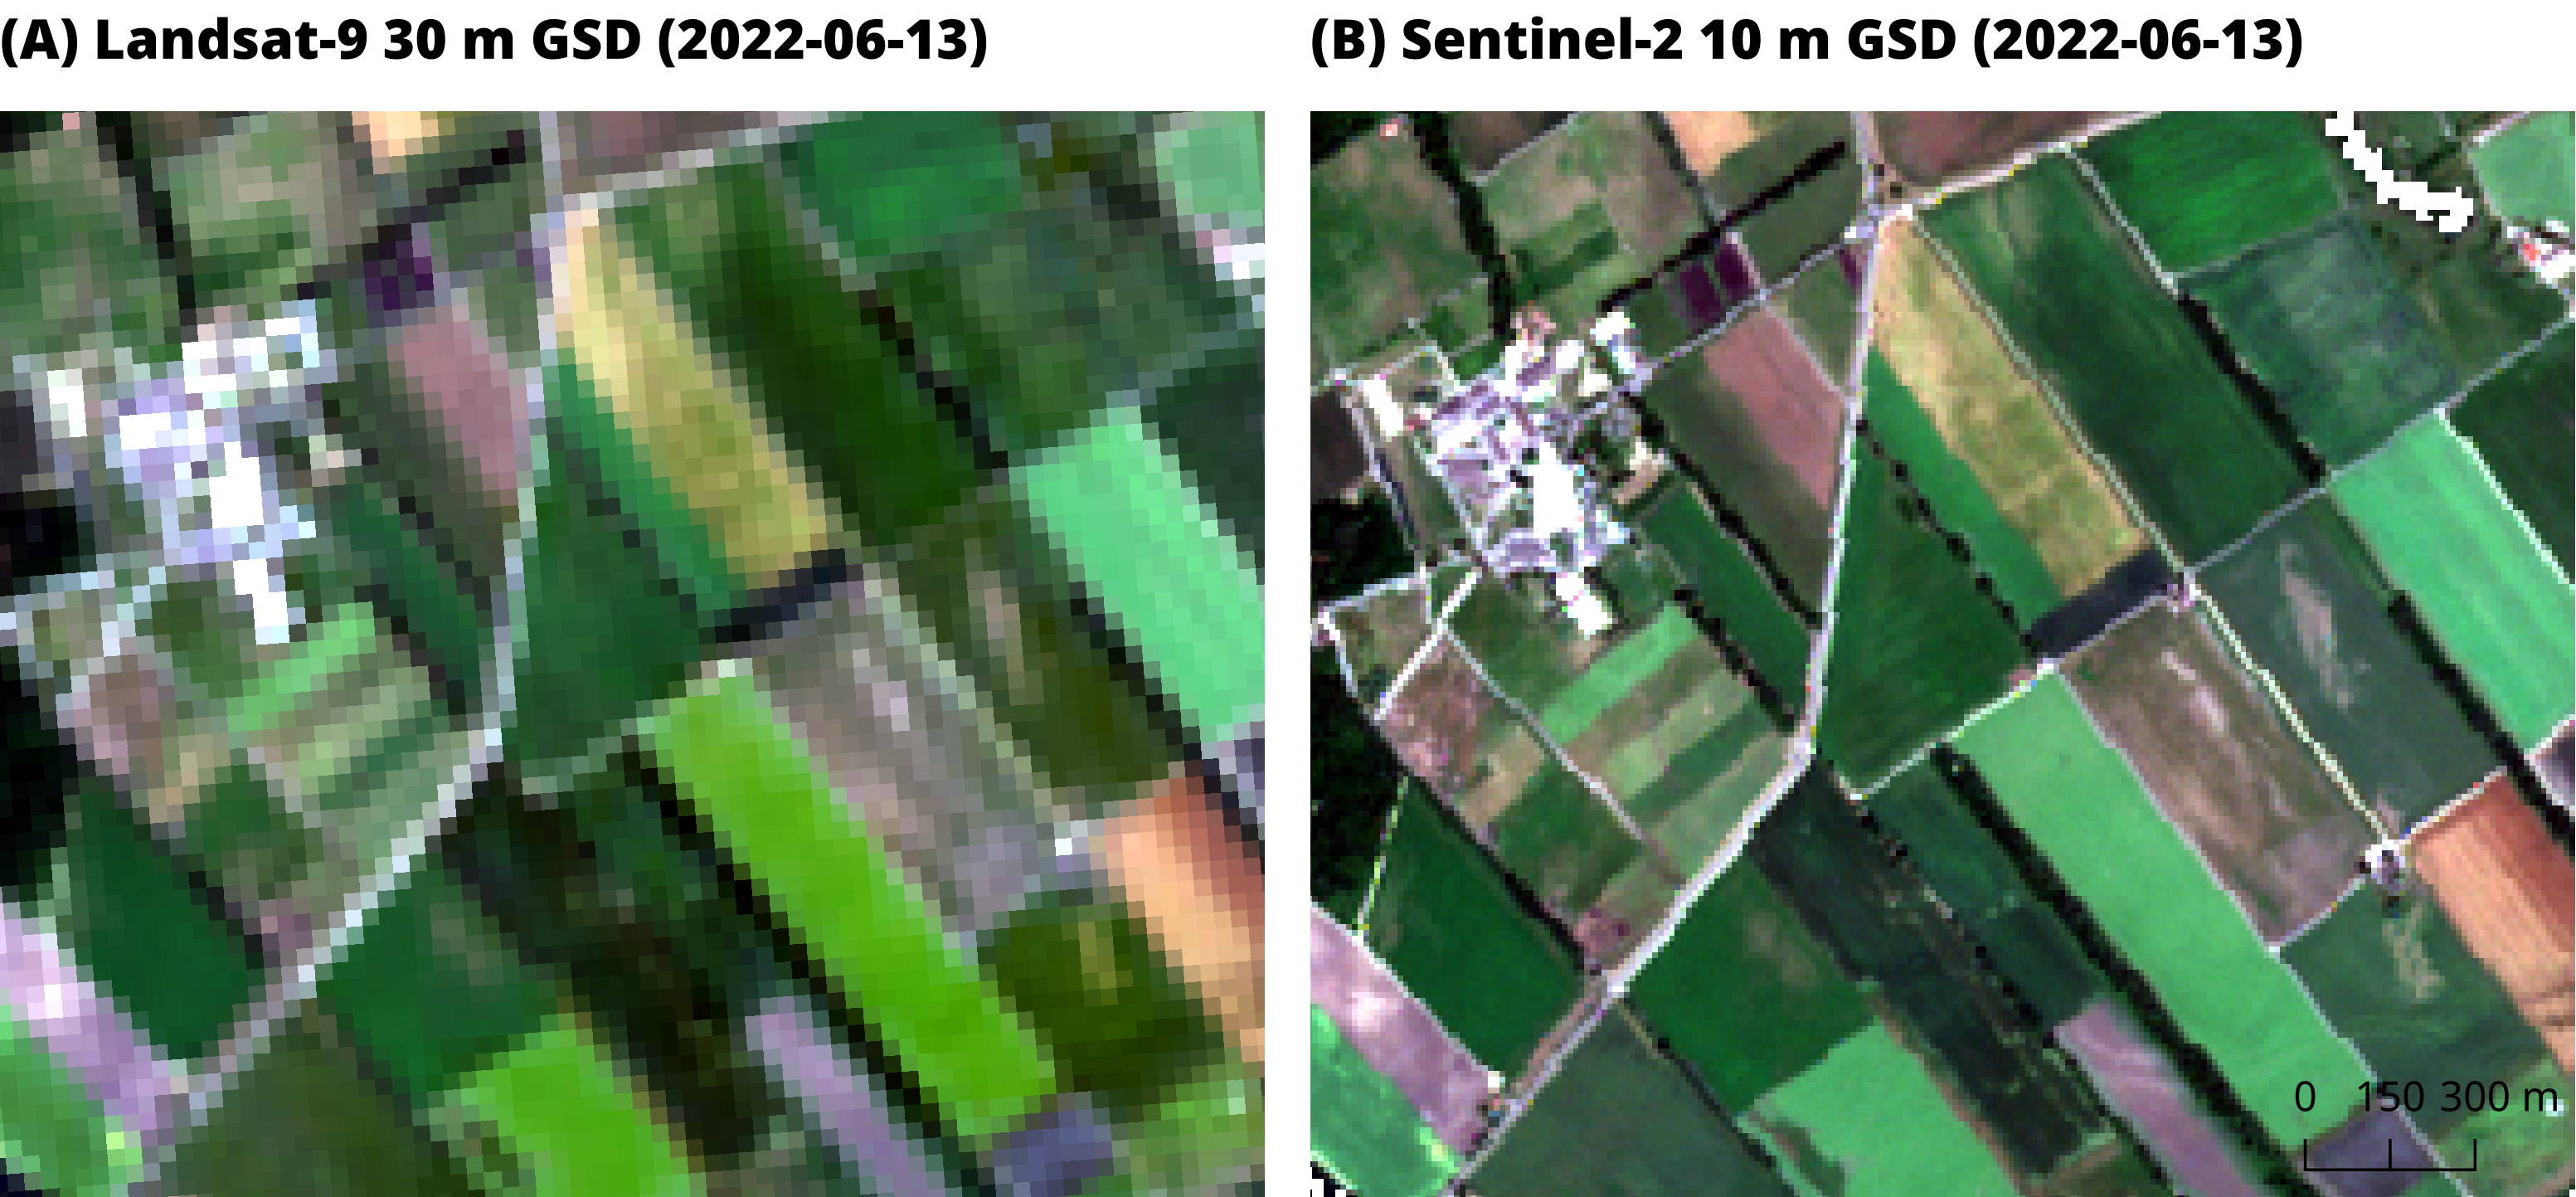
\includegraphics[width=\textwidth]{07-Discussion/img/comparison_l9-s2_witzwil22.png}
    \caption{Comparison of true-colour Landsat-9 30 m ground-sampling distance (GSD) and Sentinel-2 10 m GSD imagery acquired on 2022-06-13 of agricultural areas around Witzwil, Switzerland.}
    \label{fig:discussion-l9-vs-s2}
\end{figure}

\subsection{What are the limiting factors?}
In the Chapters \ref{chap:insights} and \ref{chap:drc} air temperature is considered as the main driver of plant growth. By growth we mean the increase in \gls{GLAI} which -- during the \gls{SE} period -- correlates with the accumulation of dry matter, i.e. dry biomass (see Figure \ref{fig:ww-growth-development} and \cite{aase_relationship_1978}). \cite{monteith_climate_1977} points out that changes in leaf area are mainly controlled by temperature and soil water availability. In Vilma Rantanen's bachelor's thesis, it was suggested that differences in \gls{GLAI} dynamics between years could be explained by precipitation patterns. This is in line with preliminary research by Hanna Sjulgård (personal communication) on the effects of drought on \gls{GLAI} dynamics in winter wheat in Sweden. Situations where wheat growth is water limited may become more relevant in the future due to climate change, even in Switzerland \citep{holzkamper_spatial_2015}. Currently, the prototype does not consider soil water availability, as this covariate is more difficult and costly to measure and is therefore often missing at larger spatial scales. Remotely sensed topsoil moisture \citep{lobell_moisture_2002, sadeghi_optical_2017} and hydrological modelling of surface water and energy balance \citep{penman_natural_1948, priestley_assessment_1972, shuttleworth_simplified_1978} could provide this information at larger spatial scales. However, the question remains whether leaf area dynamics are more controlled by temperature or water availability, as high temperatures tend to decrease soil moisture. This decrease is due to positive, non-linear feedback loops between air temperature, water vapour pressure deficit, evapotranspiration, soil moisture and temperature, and latent and sensible heat fluxes \citep{webber_diverging_2018, garcia-garcia_soil_2023}. Thus, further research on the ecophysiological processes governing the plant-soil-atmosphere continuum to identify the limiting factors for crop growth in terms of \gls{GLAI} dynamics at the landscape scale seems promising to uncover the underlying mechanisms. Another question that, to the best of our knowledge, remains largely unanswered is the effect of water availability on phenology.

An additional environmental covariate not considered in this thesis is global radiation, more specifically the fraction of absorbed \gls{PAR}, FAPAR. \cite{monteith_climate_1977} suggests modelling dry matter accumulation in terms of absorbed radiation and the efficiency with which the input solar radiation is converted into carbohydrates. The amount of radiation absorbed in turn depends on leaf area dynamics, the drivers of which have been outlined above. In an attempt to provide a unified formalism for describing crop growth in terms of leaf area \textsl{and} biomass throughout the crop development cycle, \cite{goudriaan_mathematical_1990} developed a prototype of what would become light use efficiency models \citep{gitelson_productivity_2015}. Apart from these considerations, too little radiation during meiosis, i.e. the production of gametes with the correct number of chromosomes, could lead to sterile flowers and thus reduce grain yield in winter wheat. Lack of radiation during meiosis, which occurs during booting (\gls{BBCH} macro stage 40), caused significant yield losses in France in 2016 \citep{le_gouis_how_2020}. This finding is in line with results from Spain and Mexico in spring durum \citep{villegas_daylength_2016}. To provide a more sophisticated perspective on leaf area and dry matter characteristics and ultimately grain yield, the use of light use efficiency models such as \gls{SAFYE} \citep{duchemin_simple_2008, ma_wheat_2022} therefore seems promising as the next evolutionary step of the prototype.

Finally, the effects of management on plant growth and development, such as fertilisation, pesticides and growth regulators, should not be forgotten. This actually addressed the central question of whether M or E is more central at the landscape scale, i.e. whether plant growth and development is mainly driven by environmental covariates or farm management decisions.

\subsection{How to represent time?}

Time is an essential component in the description of dynamic processes such as growth and development. The choice of time axis is therefore critical, especially as there are different possibilities for plants. From an agronomic perspective, \gls{DAS}, \gls{GDD}s and \gls{BBCH} stages are commonly chosen time axes. However, from the remote sensing data, calendar dates are inevitably the first choice. As shown in Chapter \ref{chap:phemology}, \gls{DAS}, like calendar dates, are not very meaningful, as phenological development varies greatly from year to year and also shows great spatial variability within small spatial units. \gls{GDD}s take into account the temperature dependence of plant growth, as mentioned above, and can also be used to narrow down phenological macro-stages (see Chapter \ref{chap:insights}). In addition, \cite{amin_-season_2024} achieved improved accuracy for in-season grain yield prediction using \gls{GDD}s compared to calendar dates. However, the disadvantage of \gls{GDD}s is that they only work if the exact sowing date is known, which is often not the case. In addition, the link from \gls{GDD}s to phenological development is implicit rather than explicit as with \gls{BBCH} stages, which can make communication and comparability difficult. \gls{BBCH} stages, on the other hand, are only partially covered by the \gls{WOFOST} model used in Chapter \ref{chap:phemology} (e.g. \gls{BBCH} 59 for end of heading) and would therefore require a more sophisticated phenological model. While the \gls{BBCH} scale allows a clear description of development, it cannot fully account for growth within a developmental stage: For example, at \gls{BBCH} 23 in wheat, three tillers are visible. However, multiple growth records, such as increases in leaf area or canopy cover, can now be recorded while there are still three tillers visible, i.e. the development stage remains the same. From a modelling perspective, this behaviour of the \gls{BBCH} and other scales is often not desirable.
 
In short, the choice of timescale that operates at the landscape scale, where detailed management information is often lacking, merits further scientific consideration. Ideally, the timescale would provide an explicit description of growth \textsl{and} development, i.e. the timescale should be an analytical function that assigns each timestamp ($x$) to a single trait value ($y$), and each $x$ value can be assigned a distinct stage of phenological development such as a \gls{BBCH} stage. However, such an ideal timescale does not seem to exist (yet), so further research is needed.

\section{Outlook}
In addition to the open scientific questions outlined in Section \ref{sec:disc-open-questions}, which seem worth pursuing, there are some concrete ways in which the work on the landscape-scale phenotyping prototype for quantifying winter wheat growth and development could be continued. These include extension to phenological phases not covered in this work, extension to other staple crops, and coupling with climate change projections.

\paragraph{Extend to further phenological phases}
The \gls{SE} period is preceded by leaf development and tillering, in which, for example, frost damage \citep{tschurr_frost_2023} plays a crucial role. Growth conditions during these early developmental stages therefore set the initial conditions on which \gls{SE} can build. In terms of yield formation, growth conditions during the \gls{SE} period determine the \textsl{potential} yield, while conditions during flowering and senescence, such as stay-green \citep{thomas_stay-green_2014}, determine the \textsl{actual} yield. Quantification of growth and development at all stages is therefore essential to develop a truly holistic understanding of winter wheat growth and development at the landscape scale and to make accurate yield estimates. In addition, remotely sensed \gls{GLAI} estimates could be used to determine the timing of physiological maturity, which is critical information for assessing the optimum timing of harvest.

\paragraph{Expansion to other crops}
Besides winter wheat, the prototype framework can be extended to other cereals such as rye, barley, maize or rice. Calibration data, e.g. from variety trials, will be needed to parameterise the phenological model and the \gls{DRC}s. With the main cereals covered, the prototype could then be extended to legumes such as soybean or peas and oilseeds. This will allow the most important stable crops to be covered on a global scale, making an important contribution to food security.

\paragraph{A look into the future -- climate change projections}
The thesis used measured air temperatures. To study future climate change and its effects on crop growth and development, measured meteorological covariates can be replaced by outputs from climate models. These allow the effects of different climate change scenarios on agricultural production to be simulated, thus providing an important decision-making tool for agricultural stakeholders. Ultimately, climate change projections can be used to help transform agricultural systems to reduce environmental impacts and increase resilience to provide sufficient and healthy food today, tomorrow and for all.
